\chapter{Introduction}


\section{Brief Context for the Problem}

The Domain Name System (DNS), as seen in Figure \ref{fig:dnsIntro}, translates domain names into IP addresses. This will definitely affect the daily digital interaction of each user, along with the smooth running of the Internet. Unfortunately, this one is not resistant to abuse. Meanwhile, malicious actors use DNS domains for a variety of abusive and sometimes illegal activities, such as sending malware, phishing websites, and controlling botnets \cite{so2022}. Therefore, such activity undermines the reliability and security of the Internet, posing very serious risks to cybersecurity and user trust \cite{bayer2022}. Addressing this issue requires a robust response from DNS infrastructure providers, including registrars and registries, who play a role in the management of abuse complaints. Registries refer to organisations that function to manage the top-level domains (TLDs) of the Internet, such as ".com" and ".net". On their part, registrars play a role as some form of intermediaries in the sale of domain names to the members of the public. Entities of this kind have the power to disable or deny the registration of DNS names that have been found to be abusive. But it will also consider proactive measures, such as turning down registrations that may facilitate "typosquatting", and potentially regulating permissible domain names to censor registration or renewal based on content. This would enhance the efficiency of such interventions since they shall have been transparent on the measures and the justification thereof. Although the trend is in a manner that issuing transparency reports would be able to shed light on the practices, this happens on rare occasions.

\begin{figure}[H]
    \centering
    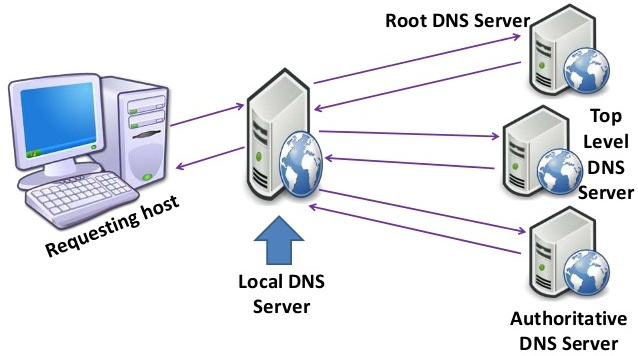
\includegraphics[width=0.4\linewidth]{introduction/dnsWork.jpg}
    \caption{How DNS works. Adapted from \cite{blanche2018understandingDNS}. }
    \label{fig:dnsIntro}
\end{figure}

\section{Motivation}

 The abuse of DNS for abusive, sometimes illegal activities, such as confusable domains and phishing, has raised questions about the integrity and security of the Internet, as depicted in the figure \ref{fig:dnsintro2} below. The severity and frequency of these concerns are highlighted in recent studies, such as the "Study on Domain Name System (DNS) Abuse: Technical Report" by Bayer et al \cite{bayer2022}, highlighting the importance of more monitoring and mitigation tactics. Not only have significant cases of DNS abuse endangered user security, but they have also damaged the general trust in the digital economy. Users' trust in online services declines as they become more aware of these hazards, necessitating the implementation of mitigation measures to regain confidence and guarantee a secure online experience. According to Hesselman et al. \cite{hesselman2020}, the idea of a "responsible Internet" aims to increase confidence and sovereignty by improving network-level transparency and accountability. Furthermore, Mathew and Cheshire's \cite{mathew2016} study "Trust and Community in the Practice of Network Security" dives into the significance of trust connections and communities in cybersecurity, demonstrating the negative effects of DNS abuse on user trust.

\begin{figure}[H]
    \centering
    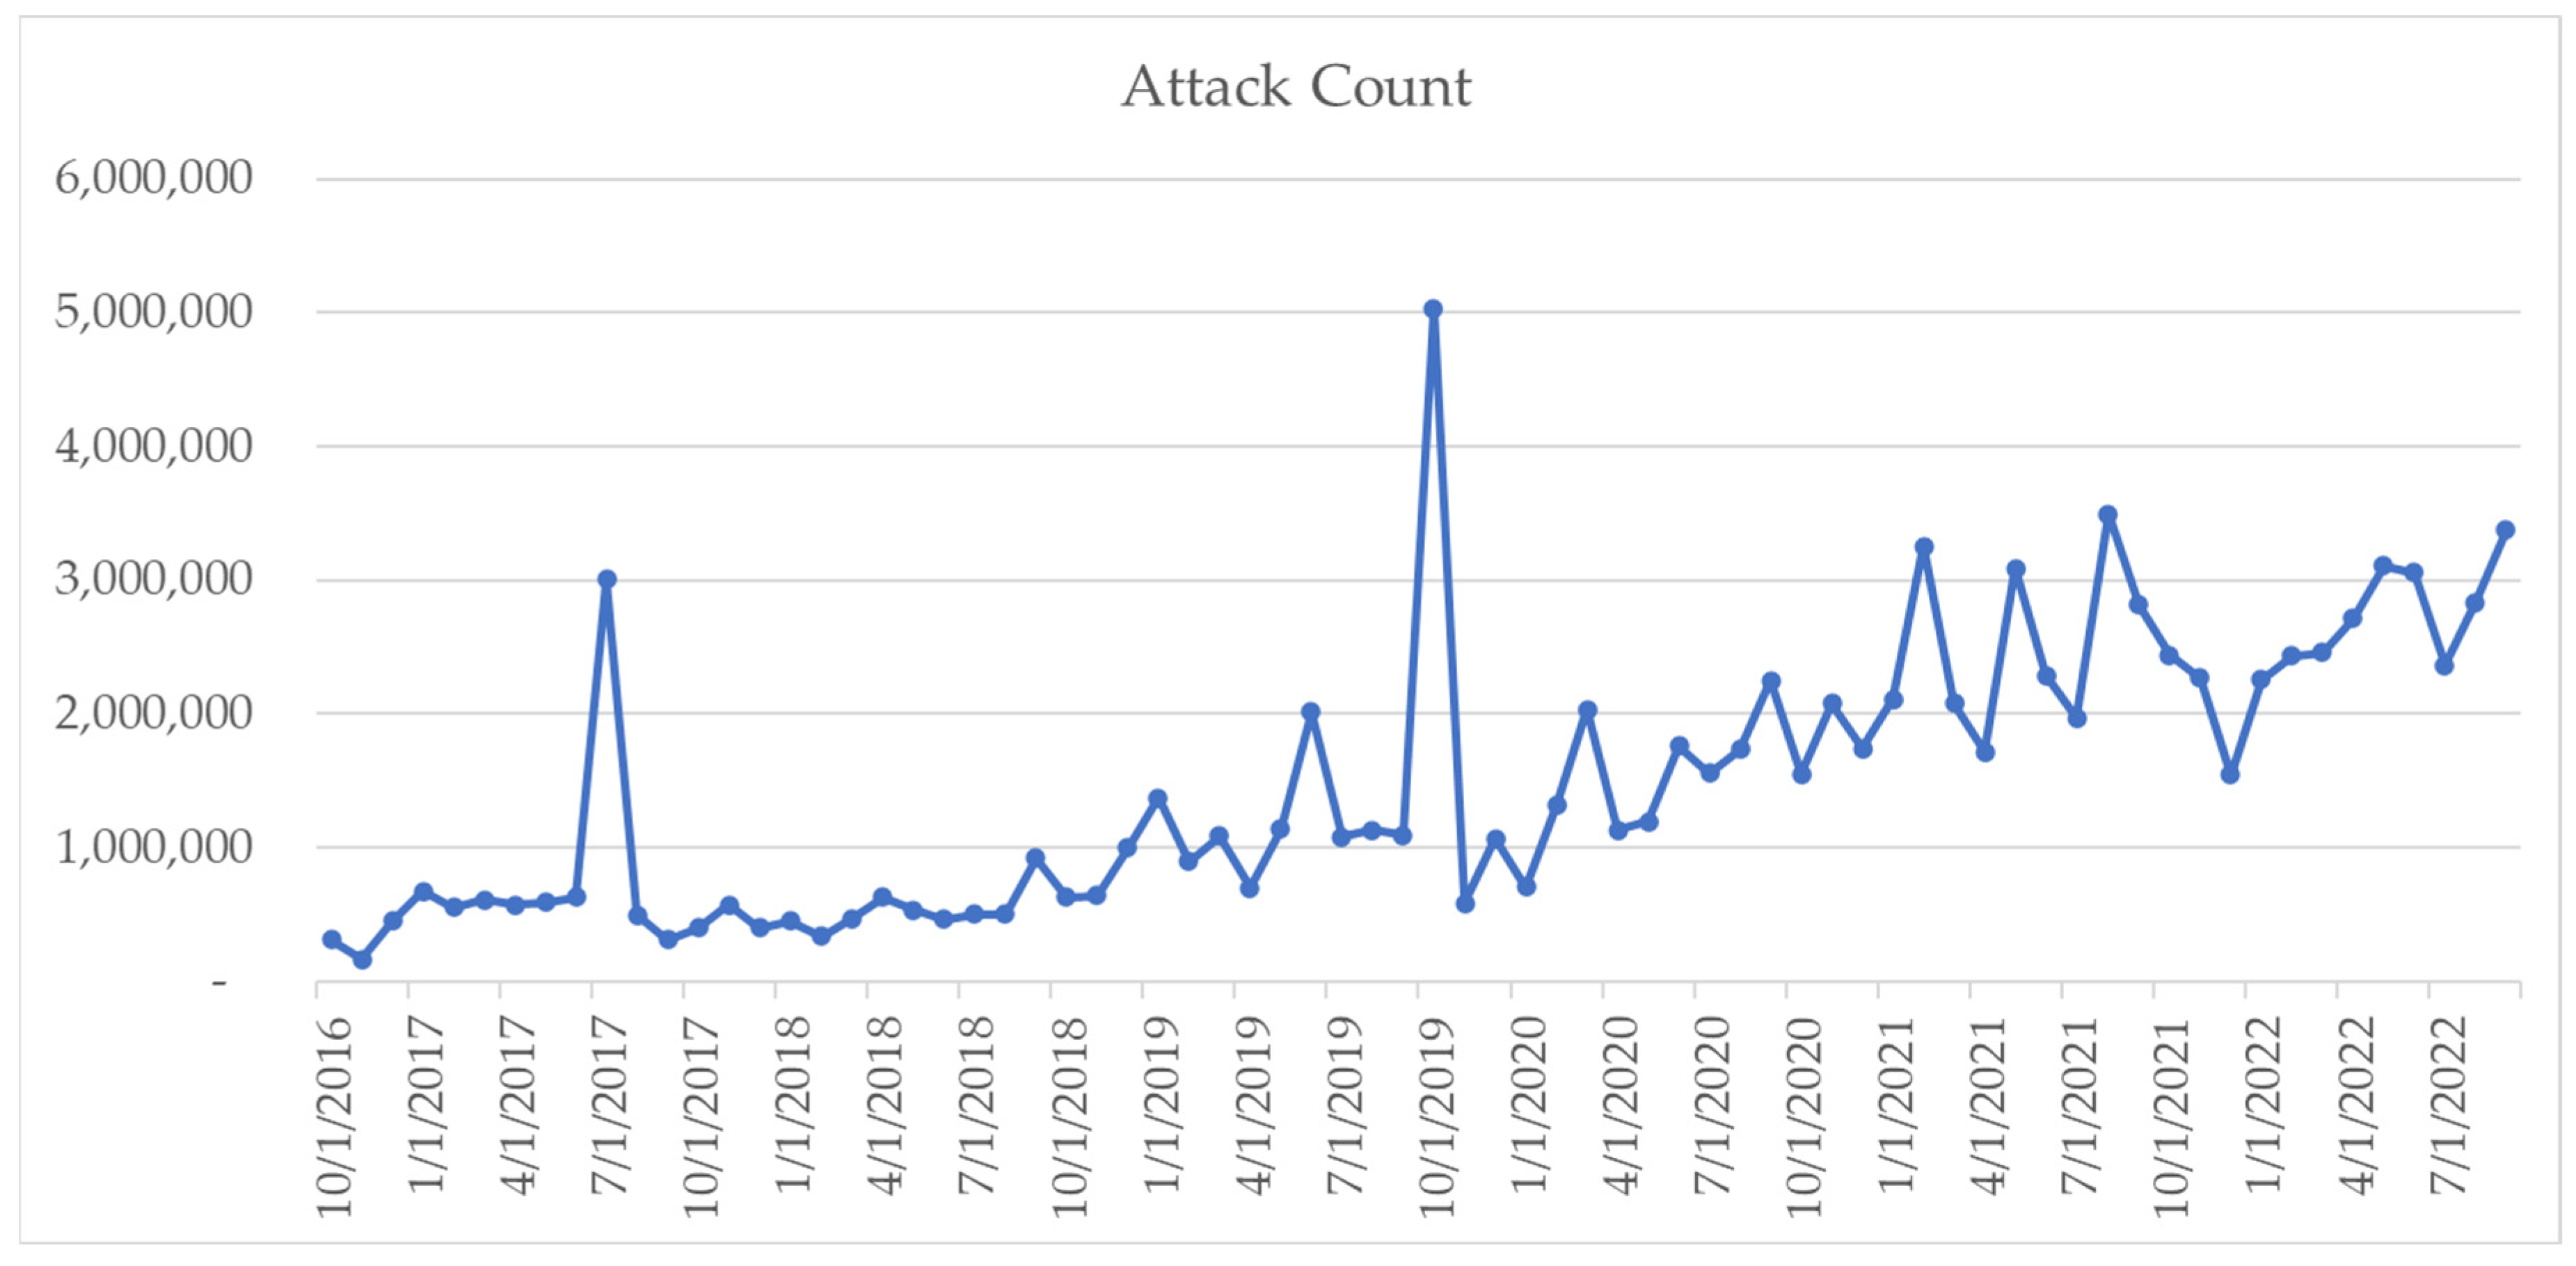
\includegraphics[width=0.5\linewidth]{introduction/maliciousActivity.png}
    \caption{ increase in DNS abuse incidents over time. Adapted from \cite{Rich2023Cyberpsychology}.}
    \label{fig:dnsintro2}
\end{figure}

Registries and registrars are leading the way in this issue, especially DNS infrastructure providers such as registrars and registries. However, their policies are probably clear and transparent to themselves, just not to outsiders.  This clear approach in handling DNS abuse allegations and its accompanying actions worsens the continuous lack of confidence. Identified in relation to this matter are the credibility and a necessary need to protect the Internet \cite{cerf2022}. It also covers the moral and legal implications, in addition to technical aspects of DNS abuse and how one can mitigate it. This is the void to which the project is motivated to fill by exploring ways to increase the transparency of mitigation of DNS abuse. To understand current efforts, the research also sought to find the difficulties in the way of more transparent practices through an evaluation of the current landscape on transparency reports and practices among DNS infrastructure providers. The ultimate goal is to provide a contribution to a system that can facilitate, promote, and enable better and more efficient approachable transparency in mitigation for DNS abuse.


\section{Research Question/Project \& Personal objective} 
\subsection{Research Question}

The primary research question for this project is: "How do the strategies and practices employed by registries, registrars, and other DNS infrastructure participants, as reflected in their transparency reports, contribute to mitigating DNS abuse, and what can these approaches teach us about developing best practices for transparency in handling DNS abuse complaints?". This question seeks to uncover the mechanisms, policies, and practices in place to mitigate DNS abuse and to what extent these efforts are transparent to the public and stakeholders.

\subsection{Project Objectives}

Assess handling of abuse complaints

\begin{itemize}
  \item Investigate the procedures and policies that DNS infrastructure providers have in place to handle abuse complaints.
  \item Document the types of DNS abuses that are most frequently reported and the response strategies used.
\end{itemize}

Assess Transparency Levels:

\begin{itemize}
  \item Analyse the current state of transparency in the actions taken by providers against DNS abuse.
  \item Identify what information is made public, how it is communicated, and the frequency of disclosure.
\end{itemize}

Evaluating Against Best Practices:

\begin{itemize}
  \item Compare the findings with best practices in the industry to identify areas of strength and opportunities for improvement.
  \item Highlight exemplary cases of transparency and effective abuse mitigation.
\end{itemize}

Develop recommendations :

\begin{itemize}
  \item Propose actionable recommendations for DNS infrastructure providers to improve their abuse handling and transparency.
  \item Suggest policy changes or initiatives that could standardise and improve practices in the industry.
  \item Feed into future work on ways in which best practices for transparency could be developed.
\end{itemize}

Contribute to stakeholder understanding: 

\begin{itemize}
  \item Provide insights that help stakeholders, including users, policymakers, and other providers, understand the landscape of DNS abuse handling and transparency.
  \item Offer a foundation for further research and discussion on improving DNS security and trust.
\end{itemize}

\section{Scope}	
The Scope of this project will consider the transparency measures that registrars and registries take to mitigate DNS abuse. It will look at the collection and characterisation of transparency reports that can be obtained from registry and registrars, among others that are given the same responsibilities to mitigate abuse. Furthermore, this work will review the reports on transparency developed within the current year, thus forming future work on the ways through which practices for transparency could be developed. The project discusses with different actors, as summarised in figure \ref{fig:dnsintrointro}, in the DNS ecosystem to obtain their opinions and insights on what they are currently practising and the challenges they face. This will involve establishing criteria that can be used to measure the way that the same transparency can affect the perception by the Internet user, which then relates to trust and safety. The new system will not include creating new transparency tools or systems, but rather will be based on scrutiny of the current procedures and recommending changes for the better. The key objective of the study is to learn more about transparency and its impacts.  

\begin{figure}[H]
    \centering
    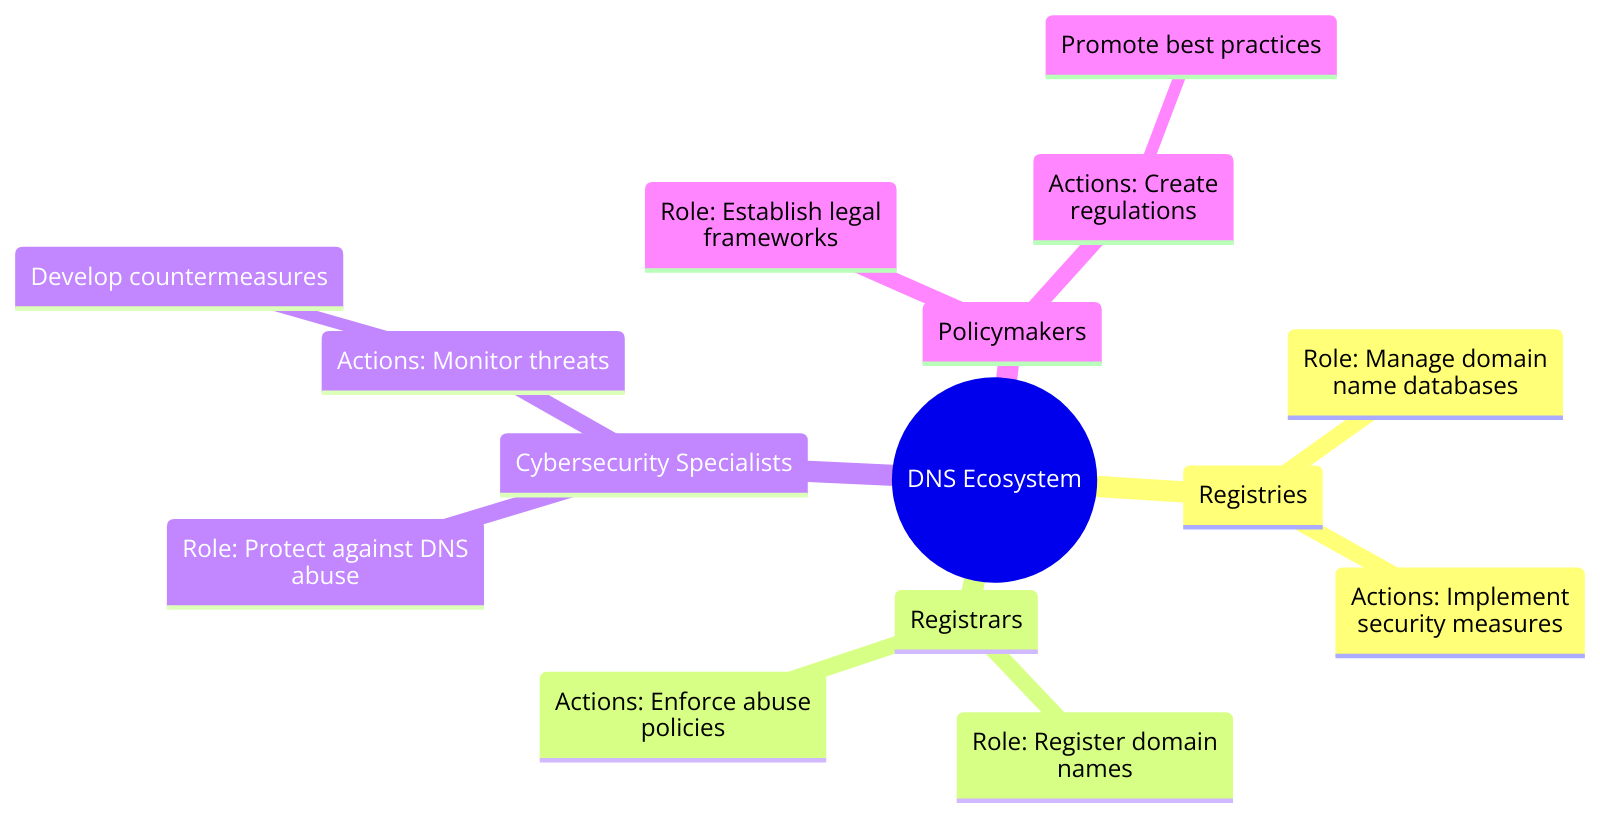
\includegraphics[width=0.7\linewidth]{introduction/diagram (8).png}
    \caption{ DNS ecosystem.}
    \label{fig:dnsintrointro}
\end{figure}

\section{ Outline of the Project Work} 

The goal of this project, "DNS Abuse Transparency", is to better understand and increase the transparency of the efforts of the registrars and registries to mitigate DNS abuse. Research will first examine the different aspects of DNS abuse, such as popular forms like phishing, confusable domains, etc. and their broader consequences. 

The questionnaire will explore the scope and effectiveness of current practices implemented on the aspect of transparency in mitigating abuse associated with the DNS. At the same time, the study will also unveil the current current transparency reports that reflect the landscape, frequency, scope, and accessibility of the reports to users. Critical evaluation of the handling of DNS abuse reports forms the core of the project.

Critical evaluation of the handling of DNS abuse reports forms the core of the project. This will involve a review of proactive security controls that may be in place, procedures for mitigation, and avoidance of abusive domain registrations. Thereafter, these will be assessed in terms of how transparency influences not only user trust, but also provider reputation, and overall the effectiveness of techniques applied in mitigating abuse. The best practices in mitigating DNS abuse.

The project will discover and clarify best practices for transparency in the mitigation of DNS abuse, based on the data and insights obtained. The careful balance between security, privacy, and transparency will be taken into account by these best practices. It is under this background that the research will, therefore, with these findings in mind, develop a set of practical recommendations for the DNS infrastructure providers seeking to increase transparency for better security and, therefore, trust in the digital ecosystem.

A comprehensive timeline will guide the progress, guaranteeing an organised study of the subject. The project, upon completion, would have contributed to a collection of recommendations and considerations for further study and policy creation in this area of Internet governance. This, in turn, would give a further comprehensive understanding of where the current state of DNS abuse transparency lies.

\section{Outline of the report}

This report offers a comprehensive account of the steps performed, decisions made, and research carried out during the project's development. The format of the report is as follows:

\textbf{Chapter 2 - Background }

This chapter discusses the foundation of DNS, its importance, its weaknesses, and several types of abuse. Explaining the methods formulated in combating DNS abuse gives a specific look at the work done by ICANN and the DNS Abuse Institute.

\textbf{Chapter 3 -  State of the art }

This chapter critically looks at some of the existing strategies towards mitigation of DNS abuse and their effectiveness. This chapter will give an account of the complex relationship that international governments have with DNS and outline efforts to openness made by companies such as Google and Cloudflare. In addition to stressing the difficulties in striking a balance between user privacy and compliance requirements, the chapter emphasises the importance of DNS in internet governance. Investigate how various tactics are used and their effects on the larger online ecosystem through critical analysis.

\textbf{Chapter 4 -  Research methodology }

This chapter describes techniques to investigate DNS abuse and transparency from the infrastructure provider. The author goes on how the questionnaires were made, how the responses from stakeholders were analysed, and what kinds of DNS abuse were found. This chapter describes the methodology used to collect and examine data to understand DNS abuse reporting procedures and transparency policies.

\textbf{Chapter 5 -  Implementation }

The chapter is a practical part of the project, where all the findings are applied, especially integrating the system, the back-end, and front-end implementations, and the technologies that will make up the system. It describes how DNS data related to abuse are visualised and how the challenges in the implementation of the system are solved. This part also involves testing and validation to ensure the success of the project.

\textbf{Chapter 6 -  Evaluation \& Discussion }

This chapter evaluates the way the project meets the mitigation of DNS abuse and the improvement of transparency. It has also been used to evaluate the benefits of transparency in mitigating DNS abuse while evaluating security issues. In addition, the chapter outlines the study constraints and the level at which the project achieved its goals.

\textbf{Chapter 7 -  Conclusion }

This chapter summarises the project's results and recommendations for enhancing DNS abuse mitigation transparency. Consider the difficulties faced, the importance of continuous attempts to improve DNS security, and the possibilities for further study in this field. In conclusion, the importance of cooperation and transparency is emphasised in the fight against DNS abuse. 
